\documentclass[aspectratio=169, 11pt]{beamer}

%--- Packages ---
\usepackage{xcolor}
\usepackage{graphicx}
\usepackage{amsmath, amssymb, amsthm}
\usepackage{booktabs}
\usepackage{tikz}
\usetikzlibrary{shapes, arrows.meta, positioning, patterns}
\usepackage{tcolorbox}
% Use standard fonts instead of fontspec/custom fonts
\usepackage[T1]{fontenc}
\usepackage{lmodern} % Latin Modern (Standard clean LaTeX font)
\usepackage{palatino} % Uses Palatino for text (similar serif style)

%--- Color Palette (Academic/Minimalist) ---
\definecolor{DeepNavy}{HTML}{002b36}
\definecolor{AccentRed}{HTML}{A52A2A}
\definecolor{TextGrey}{HTML}{333333}
\definecolor{OffWhite}{HTML}{FAFAFA}

%--- Beamer Theme Customization ---
\setbeamercolor{background canvas}{bg=OffWhite}
\setbeamercolor{normal text}{fg=TextGrey}
\setbeamercolor{frametitle}{fg=AccentRed}
\setbeamercolor{title}{fg=DeepNavy}
\setbeamercolor{structure}{fg=DeepNavy}

\setbeamertemplate{navigation symbols}{}
\setbeamertemplate{headline}{} 
\setbeamertemplate{footline}[frame number]

% Custom Frametitle
\setbeamertemplate{frametitle}{
    \vspace{0.5cm}
    \textbf{\Large\insertframetitle}\par
    \vspace{0.2cm}
}

% Custom Title Page
\setbeamertemplate{title page}{
    \vspace{2cm}
    {\huge\bfseries\color{DeepNavy}\inserttitle\par}
    \vspace{0.5cm}
    {\Large\color{AccentRed}\insertsubtitle\par}
    \vspace{1cm}
    {\large\insertauthor\par}
    \vspace{0.2cm}
    {\footnotesize \insertinstitute\par}
    \vspace{0.5cm}
    {\small \insertdate\par}
}

%--- Logo Configuration (Top Right) ---
\addtobeamertemplate{headline}{}{%
    \begin{tikzpicture}[remember picture,overlay]
        \node[anchor=north east, xshift=-0.5cm, yshift=-0.3cm] at (current page.north east) {
            % REPLACE 'example-image' WITH YOUR FILENAME (e.g., logo.png)
            \includegraphics[height=1.2cm]{image_2026-01-10_215546696.png} 
        };
    \end{tikzpicture}
}
\setbeamertemplate{caption}[numbered]

%--- Metadata ---
\title{Design and Pattern Analysis of Frequency Hopping System}
\author{Göksun Güney Küçük}
\institute{Dept. of Electrical and Electronics Engineering, Boğaziçi University}
\date{January 12, 2026}

\begin{document}

%--- Slide 1: Title ---
\begin{frame}
    \titlepage
\end{frame}

%--- Slide 2: Outline ---
\begin{frame}{Outline}
    \tableofcontents
\end{frame}

\section{Introduction}

%--- Slide 3: Motivation ---
\begin{frame}{Introduction \& Motivation}
    \begin{itemize}
        \item \textbf{Frequency Hopping Spread Spectrum (FHSS):} A dominant method for securing military communications against jamming.
        \item \textbf{The Threat:} If an adversary can predict the next frequency hop, they can launch a "Follower Jammer" attack.
        \item \textbf{Current Security Reliance:} Security relies on the secrecy of the pseudo-random sequence (PN) generated by Linear Feedback Shift Registers (LFSRs).
        \item \textbf{Research Question:} Are classical linear generators (like Gold Codes) vulnerable to "soft" attacks via modern Deep Learning?
    \end{itemize}
\end{frame}

\section{System Analysis}

%--- Slide 4: Signal Model ---
\begin{frame}{FHSS Signal Model}
    The transmitted signal $s(t)$ is modeled as a sequence of modulated pulses:
    
    $$s(t)=\sum_{k=-\infty}^{\infty}p(t-kT_{h})\cos(2\pi f_{k}(t-kT_{h})+\theta_{k}(t)+\phi_{k})$$
    
    \vspace{1em}
    \textbf{Key Parameters:}
    \begin{itemize}
        \item $T_h$: Hop duration (dwell time).
        \item $f_k$: Carrier frequency selected from a predefined hopset.
        \item $\theta_k$: Data modulation term ($\pm \Delta f$).
    \end{itemize}
\end{frame}

%--- Slide: M-Sequences ---
\begin{frame}{M-Sequences}
    \begin{columns}
        \column{0.5\textwidth}
        \textbf{Maximal Length Sequences:}
        \begin{itemize}
            \item Generated by a single LFSR with a \textbf{Primitive Polynomial}.
            \item \textbf{Period:} $2^L - 1$.
            \item \textbf{Properties:} Good randomness, but simple linear structure.
        \end{itemize}
        
        \vspace{1em}
        \textbf{Project Polynomial ($P_1$):}
        $$ P_1(x) = 1 + x^3 + x^{10} $$
        \begin{itemize}
            \item Degree $L=10$.
            \item Taps at bits 3 and 10.
        \end{itemize}

        \column{0.5\textwidth}
        \centering
        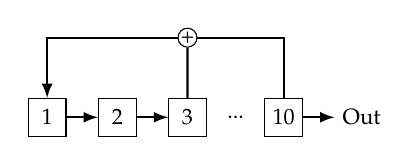
\begin{tikzpicture}[node distance=0.5cm, scale=0.8, transform shape]
            \tikzstyle{bit} = [draw, rectangle, minimum size=0.6cm, align=center]
            \tikzstyle{xor} = [draw, circle, inner sep=0pt, minimum size=0.3cm]
            \tikzstyle{line} = [draw, thick, -latex]
            
            % LFSR Cells
            \node[bit] (b1) {1};
            \node[bit, right=of b1] (b2) {2};
            \node[bit, right=of b2] (b3) {3};
            \node[right=0.2cm of b3] (dots) {...};
            \node[bit, right=0.2cm of dots] (b10) {10};
            
            % XOR Gate
            \node[xor, above=0.8cm of b3] (x1) {+};
            
            % Connections (Shift)
            \draw[line] (b1) -- (b2);
            \draw[line] (b2) -- (b3);
            
            % Feedback Taps
            \draw[thick] (b10.north) |- (x1.east); % Tap from 10
            \draw[thick] (b3.north) -- (x1.south);             % Tap from 3
            
            % Feedback Return
            \draw[line] (x1.west) -| (b1.north); % Back to 1
            
            % Output
            \draw[line] (b10.east) -- ++(0.5,0) node[right] {Out};
        \end{tikzpicture}
    \end{columns}
\end{frame}

%--- Slide: Gold Codes ---
\begin{frame}{Gold Codes}
    \begin{columns}
        \column{0.5\textwidth}
        \textbf{Gold Code Construction:}
        \begin{itemize}
            \item Formed by the XOR sum of two "Preferred Pair" M-sequences.
            \item \textbf{Advantage:} Large family of codes with low cross-correlation.
            \item \textbf{Linear Complexity:} $2L$ (Much harder to crack than $L$).
        \end{itemize}
        
        \vspace{1em}
        \textbf{Project Configuration:}
        \begin{itemize}
            \item $poly_1 = 1 + x^3 + x^{10}$
            \item $poly_2 = 1 + x^7 + x^{10}$
            \item Output: $G(t) = m_1(t) \oplus m_2(t)$
        \end{itemize}

        \column{0.5\textwidth}
        \centering
        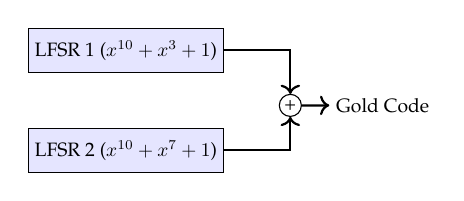
\begin{tikzpicture}[node distance=1cm, scale=0.7, transform shape]
            \tikzstyle{lfsr} = [draw, rectangle, minimum width=3cm, minimum height=0.8cm, fill=blue!10]
            \tikzstyle{xor} = [draw, circle, inner sep=0pt, minimum size=0.4cm]
            
            \node[lfsr] (l1) {LFSR 1 ($x^{10}+x^3+1$)};
            \node[lfsr, below=1cm of l1] (l2) {LFSR 2 ($x^{10}+x^7+1$)};
            
            \node[xor, right=1cm of l1, yshift=-1cm] (sum) {+};
            
            \draw[->, thick] (l1.east) -| (sum);
            \draw[->, thick] (l2.east) -| (sum);
            
            \node[right=0.5cm of sum] (out) {Gold Code};
            \draw[->, thick] (sum) -- (out);
        \end{tikzpicture}
    \end{columns}
\end{frame}

%--- Slide 5: The Mathematical Vulnerability ---
\begin{frame}{The Vulnerability of Linear Generators}
    \begin{tcolorbox}[colback=OffWhite, colframe=DeepNavy, title=Linear Complexity]
    For a Gold Code generated by two degree-$n$ polynomials, the linear complexity is exactly $2n$. Observing $2n$ bits theoretically allows solving for the future sequence.
    \end{tcolorbox}
    
    \begin{itemize}
        \item \textbf{Classical Attack:} Berlekamp-Massey Algorithm.
        \item \textbf{Limitation:} Algebraic attacks are brittle. A single bit error causes the calculated complexity to explode.
        \item \textbf{The AI Approach:} Deep Learning offers a "soft" attack surface, potentially learning from noisy spectrograms without explicit demodulation.
    \end{itemize}
\end{frame}




%--- Slide 7: Spectrogram Analysis ---
\begin{frame}{Spectrogram of FHSS}
    The Short-Time Fourier Transform (STFT) provides the "Vision" input for the neural network.
    
    \begin{figure}
        \centering
        % Use demo option to simulate image if you don't have one
        \includegraphics[width=0.8\textwidth, height=4cm]{full_signal_stft_snr_0dB.png} 
        \caption{Spectrogram of received FHSS signal in 0 dB AWGN.}
    \end{figure}
\end{frame}

\section{Deep Learning Methodology}

%--- Slide: Dataset Generation Strategy ---
\begin{frame}{Dataset Generation Strategy (Disjoint Pools)}
    To strictly evaluate generalization (algebraic learning) vs. memorization, we employed a \textbf{Seed-Based Splitting} strategy in Python.
    
    \begin{tcolorbox}[colback=blue!5, colframe=blue!40, title=The "Pool" Logic (\texttt{generate\_dataset.py})]
    Instead of splitting random time samples, we split the \textbf{Generator Seeds}.
    \begin{enumerate}
        \item \textbf{Universe of Seeds:} All non-zero 10-bit states ($2^{10}-1 = 1023$ seeds).
        \item \textbf{Shuffling:} The seeds are randomly shuffled to remove any structural bias.
        \item \textbf{Strict Partitioning:}
        \begin{itemize}
            \item \textbf{Training Pool (70\%):} $\approx 716$ seeds. The model sees the "Universe" from these starting points.
            \item \textbf{Validation Pool (15\%):} $\approx 153$ seeds. 
            \item \textbf{Test Pool (15\%):} $\approx 153$ seeds. 
            Zero leakage between Train, Val, Test sets.
        \end{itemize}
    \end{enumerate}
    \end{tcolorbox}
    \vspace{0.5em}
\end{frame}

\begin{frame}{Dataset Composition}

    \begin{columns}
        \column{0.5\textwidth}
        \textbf{Dataset Composition:}
        \begin{itemize}
            \item \textbf{SNR Levels:} 11 Levels (-10 dB to +10 dB, step 2 dB).
            \item \textbf{Total Signals:} $1023\times11$ full transmissions. 50 hops per transmission.
        \end{itemize}
        
        \column{0.5\textwidth}
        \textbf{Scale:}
        \begin{itemize}
            \item \textbf{Total Labeled Hops:} $>560,000$ examples.
            \item \textbf{Storage:} HDF5 Format ($\approx 6 GB$).
        \end{itemize}
    \end{columns}
        
\end{frame}


%--- Slide: Sequence Preparation ---
\begin{frame}{Sequence Preparation \& Windowing}
    The raw spectrograms must be converted into supervised learning pairs $(X, y)$.
    \vspace{2mm}
    \begin{columns}
        \column{0.6\textwidth}
        \textbf{Sliding Window Logic:}
        \begin{itemize}
            \item \textbf{Lookback Window ($W$):} The model sees $W$ past hops.
            \item \textbf{Input ($X_t$):} A tensor of shape $(W, 1024, 3)$.
            \item \textbf{Target ($y_t$):} The discrete index of the \textbf{Next Hop} ($t+1$).
        \end{itemize}
        
        \vspace{1em}
        \textbf{Index-Based Loading:}
        To handle the massive dataset (GBs of spectrograms), we only store the \textbf{Start Indices} in RAM. The DataLoader fetches the heavy 2D images on-the-fly from the HDF5 archive.
        
        \column{0.4\textwidth}
        \centering
        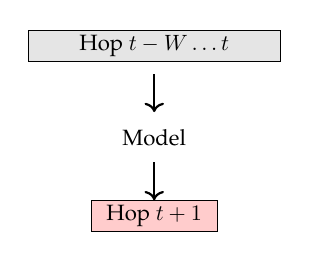
\begin{tikzpicture}[scale=0.8, transform shape]
            \draw[fill=gray!20] (0,0) rectangle (4,0.5) node[midway] {Hop $t-W \dots t$};
            \draw[->, thick] (2, -0.2) -- (2, -0.8);
            \node at (2, -1.2) {Model};
            \draw[->, thick] (2, -1.6) -- (2, -2.2);
            \draw[fill=red!20] (1, -2.7) rectangle (3, -2.2) node[midway] {Hop $t+1$};
        \end{tikzpicture}
    \end{columns}
\end{frame}

%--- Slide 8: Hybrid Architecture ---
\begin{frame}{Hybrid CNN-Transformer Architecture}
    We implemented a two-stage architecture to separate signal detection from cryptanalysis.
    
    \begin{enumerate}
        \item \textbf{Vision Module (CNN):} 
        \begin{itemize}
            \item Input: STFT frame (1024 bins $\times$ 3 time steps).
            \item Output: Discrete frequency index (0-7).
            \item Purpose: Performs a "Hard Decision" to isolate noise.
        \end{itemize}
        \item \textbf{Sequence Modeler (Transformer):}
        \begin{itemize}
            \item Analyzes the history of discrete hops to predict the next state.
        \end{itemize}
    \end{enumerate}
\end{frame}



\begin{frame}{Vision Module Architecture}
\usetikzlibrary{patterns}
    \begin{figure}
        \centering
        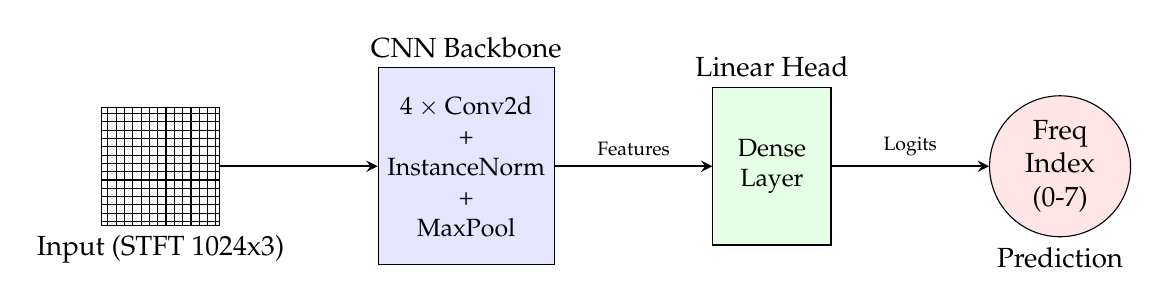
\begin{tikzpicture}[
            % INCREASED DISTANCE to prevent overlap
            node distance=2cm, 
            auto,
            % FIXED WIDTHS to ensure text fits inside
            layer/.style={
                draw, rectangle, 
                minimum height=2.5cm, 
                minimum width=2cm, 
                align=center, 
                fill=blue!10,
                font=\small
            },
            linear/.style={
                draw, rectangle, 
                minimum height=2cm, 
                minimum width=1.5cm, 
                align=center, 
                fill=green!10,
                font=\small
            },
            arrow/.style={->, thick, >=stealth}
        ]
    
        % Input
        \node[draw, rectangle, minimum size=1.5cm, pattern=grid, label=below:{Input (STFT 1024x3)}] (input) {};
    
        % CNN Stack
        \node[layer, right=of input, label=above:{CNN Backbone}] (cnn) {4 $\times$ Conv2d\\+\\InstanceNorm\\+\\MaxPool};
    
        % Linear / Classification Head
        \node[linear, right=of cnn, label=above:{Linear Head}] (dense) {Dense\\Layer};
    
        % Output Class
        \node[draw, circle, right=of dense, minimum size=1.5cm, fill=red!10, align=center, label=below:{Prediction}] (out) {Freq\\Index\\(0-7)};
    
        % Arrows
        \draw[arrow] (input) -- (cnn);
        \draw[arrow] (cnn) -- node[above, font=\scriptsize] {Features} (dense);
        \draw[arrow] (dense) -- node[above, font=\scriptsize] {Logits} (out);
    
        \end{tikzpicture}
        \caption{Vision Module Architecture}
    \end{figure}
\end{frame}


%--- Slide 9: Why Transformers? ---
\begin{frame}{Why Transformers?}
    Unlike LSTMs/RNNs which compress history into a hidden state, Transformers process the entire history window simultaneously via \textbf{Self-Attention}.
    
    \begin{tcolorbox}[colframe=AccentRed, colback=white]
    \textbf{Attention Mechanism:} Allows the model to "attend" specifically to relevant LFSR taps (e.g., $t-3$ and $t-10$) regardless of distance, solving the vanishing gradient problem for XOR operations.
    \end{tcolorbox}
\end{frame}

%--- Slide 10: Transformer Design ---
\begin{frame}{Transformer Specification}
    \begin{itemize}
        \item \textbf{Embeddings:} Discrete frequency indices mapped to vectors ($d=64$).
        \item \textbf{Positional Encoding:} Essential for relative time awareness.
        \item \textbf{Encoder:} 2 Layers, 4 Heads.
        \item \textbf{Reasoning:} 4 Heads were chosen to ensure independent attention mechanisms could track multiple feedback taps simultaneously.
    \end{itemize}
    
    \vspace{1em}
\end{frame}

\begin{frame}{Transformer Architecture}
    \begin{figure}[H]
    \centering
    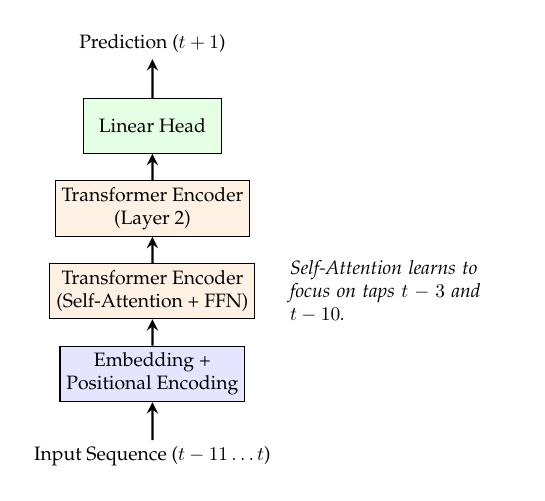
\begin{tikzpicture}[scale=0.7, transform shape, node distance=1.5cm]
        % Styles
        \tikzstyle{block} = [draw, rectangle, minimum height=1cm, minimum width=2.5cm, align=center, fill=blue!10]
        \tikzstyle{arrow} = [->, >=stealth, thick]

        % Nodes
        \node (input) {Input Sequence ($t-11 \dots t$)};
        \node [block, above of=input] (embed) {Embedding + \\ Positional Encoding};
        \node [block, above of=embed, fill=orange!10] (trans1) {Transformer Encoder \\ (Self-Attention + FFN)};
        \node [block, above of=trans1, fill=orange!10] (trans2) {Transformer Encoder \\ (Layer 2)};
        \node [block, above of=trans2, fill=green!10] (fc) {Linear Head};
        \node [above of=fc] (output) {Prediction ($t+1$)};

        % Arrows
        \draw [arrow] (input) -- (embed);
        \draw [arrow] (embed) -- (trans1);
        \draw [arrow] (trans1) -- (trans2);
        \draw [arrow] (trans2) -- (fc);
        \draw [arrow] (fc) -- (output);
        
        % Annotation
        \node [right of=trans1, xshift=3cm, text width=4cm, align=left] {\textit{Self-Attention learns to focus on taps $t-3$ and $t-10$.}};
    \end{tikzpicture}
    \caption{The Transformer-based architecture used for Neural Cryptanalysis.}
    \label{fig:transformer}
\end{figure}
    
\end{frame}

\section{Experimental Results}

%--- Slide 11: Experiment 1 - M-Sequences ---
\begin{frame}{Experiment 1: M-Sequence Control}
    \textbf{Objective:} Validate if the model can learn simple linear logic ($L=10$).
    
    \begin{itemize}
        \item \textbf{Hypothesis:} Since M-Sequences have a single cycle, training on 70\% of seeds should allow generalization to the unseen 30\%.
        \item \textbf{Result:} The model achieved \textbf{99.9\% accuracy} on the validation set.
        \item \textbf{Conclusion:} Neural Networks can approximate LFSR logic over $GF(2)$ if the state space is fully traversable.
    \end{itemize}
\end{frame}

%--- Slide 12: Sensitivity to Lookback Window ---
\begin{frame}{Observability Phase Transition}
    We varied the Lookback Window ($W$) to verify the model was performing algebraic solving, not statistical guessing.
    
    \begin{table}[]
    \centering
    \begin{tabular}{@{}llcl@{}}
    \toprule
    \textbf{Window} & \textbf{Total Bits} & \textbf{Observability} & \textbf{Accuracy} \\ \midrule
    $W=2$ & 6 bits & Under-determined & 12.5\% (Random) \\
    $W=3$ & 9 bits & Under-determined & 50.0\% (Partial) \\
    $W=4$ & 12 bits & \textbf{Fully Observable} & \textbf{99.9\% (Solved)} \\ \bottomrule
    \end{tabular}
    \caption{Impact of History Window}
    \end{table}
    
    The transition at $W=4$ matches the theoretical threshold ($\lceil 10/3 \rceil = 4$).
\end{frame}

\begin{frame}{Confusion Matrices for Varied Lookback Windows}
    \begin{figure}[H]
        \centering
        \begin{minipage}{0.32\textwidth}
            \centering
            \includegraphics[width=\linewidth]{test_mseq_confusion (3).png}
            \footnotesize \textbf{$W=2$ (12.5\%)}
            \label{W=2}
        \end{minipage}
        \hfill
        \begin{minipage}{0.32\textwidth}
            \centering
            \includegraphics[width=\linewidth]{test_mseq_confusion_lookback3.png}
            \footnotesize \textbf{$W=3$ (50.0\%)}
        \end{minipage}
        \hfill
        \begin{minipage}{0.32\textwidth}
            \centering
            \includegraphics[width=\linewidth]{test_mseq_confusion_lookback4.png}
            \footnotesize \textbf{$W=4$ (99.9\%)}
        \end{minipage}
        \caption{Confusion Matrices for M-Sequence Prediction. At $W=2$ (6 bits), the system is under-determined (random). At $W=3$ (9 bits), we are exactly 1 bit short of the 10-bit state, resulting in $\approx 50\%$ accuracy (2-way ambiguity). At $W=4$ (12 bits), the system is fully determined, achieving perfect prediction.}
        \label{fig:cm_mseq_sensitivity}
    \end{figure}
    
\end{frame}

%--- Slide 13: Experiment 2 - Gold Codes ---
\begin{frame}{Experiment 2: Gold Code Robustness}
    \textbf{Objective:} Attack Gold Codes (Degree 10, Linear Complexity 20).
    
    \begin{itemize}
        \item \textbf{Setup:} Lookback window $W=14$ (42 bits), theoretically sufficient to solve the 20-bit state.
        \item \textbf{Result:} Accuracy stalled at exactly \textbf{24.7\%}.
        \item \textbf{Observation:} A "Partial Break" occurred, but not a full solution.
    \end{itemize}
\end{frame}

\begin{frame}{Confusion Matrix of the Gold Code Experiment}
    \begin{figure}[H]
        \centering
        \includegraphics[width=0.4\textwidth]{test_gold_confusion.png}
        \caption{Confusion Matrix for Gold Code Prediction ($W=14$).}
        \label{fig:cm_gold}
    \end{figure}
    
\end{frame}

%--- Slide 14: Analysis of Gold Code Failure ---
\begin{frame}{The Parity Collapse}
    The Confusion Matrix revealed a structured failure mode.
    
    \begin{itemize}
        \item The model successfully learned the \textbf{Parity Bit}, effectively reducing the search space by half.
        \item It correctly classified signals into 4 element subgroups but could not distinguish within them, effectively predicting 1 bit of information.
        \item \textbf{Reason:} Standard Gradient Descent failed to resolve the remaining 2 bits of state due to the complexity of the "Multiverse" topology.
    \end{itemize}
\end{frame}

\section{Theoretical Discussion}

%--- Slide 15: Topological Disconnectedness ---
\begin{frame}{Why M-Sequences Break but Gold Codes Don't}
    \textbf{M-Sequences (The "Universe"):}
    \begin{itemize}
        \item Single connected cycle. Training on any segment provides global structure info.
    \end{itemize}
    
    \vspace{0.5em}
    \textbf{Gold Codes (The "Multiverse"):}
    \begin{itemize}
        \item Family of many distinct, disjoint cycles.
        \item The optimizer must learn a function that generalizes across disconnected manifolds.
        \item The model struggles to interpolate between disjoint cycles, learning only "local" statistics.
    \end{itemize}
\end{frame}

\section{Conclusion}

%--- Slide 18: Summary of Findings ---
\begin{frame}{Summary of Findings}
    \begin{table}[]
    \centering
    \begin{tabular}{@{}lll@{}}
    \toprule
    \textbf{Feature} & \textbf{M-Sequences} & \textbf{Gold Codes} \\ \midrule
    \textbf{Linear Complexity} & Low ($L=10$) & High ($L=20$) \\
    \textbf{Topology} & Single Cycle & Disjoint Cycles \\
    \textbf{DL Accuracy} & \textbf{99.9\% (Solved)} & \textbf{25\% (Partial)} \\
    \textbf{Vulnerability} & High (Structural) & Low (Robust) \\ \bottomrule
    \end{tabular}
    \caption{Comparison of Generator Vulnerabilities}
    \end{table}
\end{frame}

%--- Slide 19: Conclusion ---
\begin{frame}{Conclusion \& Implications}
    \begin{enumerate}
        \item \textbf{Experiments' Conclusion:} Simple linear sequences are structurally brittle against AI, although Gold Codes remain robust.
        \item \textbf{AI Limitations:} While universal approximators, Neural Networks fail to traverse the shattered loss landscape of high-order parity functions without specialized architectures.
    \end{enumerate}
\end{frame}
%--- References ---
\begin{frame}[allowframebreaks]{References}
    \tiny
    \begin{thebibliography}{99}

    \bibitem{proakis}
    J. G. Proakis and M. Salehi, \textit{Digital Communications}, 5th ed. New York, NY, USA: McGraw-Hill, 2008.

    \bibitem{golomb}
    S. W. Golomb, \textit{Shift Register Sequences}. San Francisco, CA, USA: Holden-Day, 1967.

    \bibitem{gold}
    R. Gold, "Optimal binary sequences for spread spectrum multiplexing," \textit{IEEE Transactions on Information Theory}, vol. 13, no. 4, pp. 619–621, Oct. 1967.

    \bibitem{massey}
    J. L. Massey, "Shift-register synthesis and BCH decoding," \textit{IEEE Transactions on Information Theory}, vol. 15, no. 1, pp. 122–127, Jan. 1969.

    \bibitem{attention}
    A. Vaswani et al., "Attention is all you need," in \textit{Advances in Neural Information Processing Systems}, 2017, pp. 5998–6008.

    \bibitem{goodfellow}
    I. Goodfellow, Y. Bengio, and A. Courville, \textit{Deep Learning}. Cambridge, MA, USA: MIT Press, 2016.

    \bibitem{gupta2021}
    S. Gupta, P. Singh, N. Shrotriya, and T. Baweja, "LFSR Next Bit Prediction through Deep Learning," \textit{Journal of Informatics Electrical and Electronics Engineering (JIEEE)}, vol. 2, no. 2, 2021.

    \bibitem{tao2025}
    T. Tao, D. Doshi, D. S. Kalra, T. He, and M. Barkeshli, "(How) Can Transformers Predict Pseudo-Random Numbers?" in \textit{Forty-second International Conference on Machine Learning (ICML)}, 2025.

    \bibitem{li2020lstm}
    G. Li, J. Xu, W. Shen, W. Wang, Z. Liu, and G. Ding, "LSTM-based Frequency Hopping Sequence Prediction," in \textit{2020 International Conference on Wireless Communications and Signal Processing (WCSP)}, Nanjing, China, 2020, pp. 472--477.

    \bibitem{kaiser2015neural}
    \L. Kaiser and I. Sutskever, "Neural GPUs Learn Algorithms," \textit{arXiv preprint arXiv:1511.08228}, 2015.

    \end{thebibliography}
\end{frame}
%--- Slide 20: Acknowledgments ---
\begin{frame}{}
    \centering
    {\Large Thank You.}
\end{frame}

\end{document}